\chapter{Software}

\section{Communication Core}
Paul -done


\section{CarControl Core}
The \textbf{CarControl Core} is responsible for processing all the data that the communications core receives from other components, and calculating the correct reactions (Motor Controller signals) to that data. 

\subsection{Location}
The CarControl Core software project resides in $software/Car2X\_carControl$; the $.sopcinfo$ file used to generate the board support package here: \\$hardware/nios\_system.sopcinfo$. The software runs on Core 1 of the system.

\subsection{Program flow}
The control core cyclically accesses the current $CarState$ from the shared memory and performs all calculations. The main loop can be broken down into four parts.

\begin{enumerate}
\item Get current $CarState$ from the shared memory (blocking).
\item Check the operating mode, $state.reqOpMode$. If a new one has been requested, the transition is performed and set in $state.currOpMode$.
\item Get the requested velocities $state.reqVel$ and transform them into goal velocities for each wheel. These are then written into $state.MotorECU\_State$.
\item Write the changed $CarState$ object back into the shared memory and release the mutex.
\end{enumerate}

\subsection{Operating modes}
A state machine is used to restrict or alter the car's behaviour, based on the current \textbf{Operating mode} of the car. Broadly speaking, an Operating Mode places restrictions on what actors can control the car at any given time, and the velocity at which the car may move. Some Operating Modes are used internally, while others can be requested by the user.

\begin{description} 
\item[PreOperational] Initial mode, used internally during the startup phase. The velocity is restricted to $0$ on all motors.
\item[Idle] This operating mode is automatically transitioned to upon successful communication with all four Motor Control ECUs. Velocity is restricted to $0$ on all motors.
\item[AutomaticDrive] This mode is to be used when the car drives autonomously. The car may only be controlled from the IP address that is registered as the autonomous driving component (the image processing component in our case). The velocity is restricted to $200mm/s$.
\item[ManualDrive] A $RemoteControlMessage$ C2X message will transition the car into this mode. Subsequently, the car may only be controlled from the IP address that sent the aforementioned message. The velocity is restricted to $400mm/s$.
\item[EmergencyStop] Triggered by an $EmergencyBrakeMessage$, this operation mode will immediately set all motor velocities to $0$, effectively executing an emergency stop. To exit this operating mode, either a $RemoteControlMessage$ must be sent.
\end{description}

\subsection{Motor velocity calculation}
The motor velocity calculations are relatively straightforward. Each operating mode has a maximum velocity that may be requested. Any velocities above this limit are scaled down to the limit. Equations \eqref{carcontrol:avel_calc} \eqref{carcontrol:vel_calc} show how the scaling is performed.

\begin{equation}
\label{carcontrol:avel_calc}
v_{limit} = \frac{1}{4} \sum_{i=1}^{4} v_i 
\end{equation}

\begin{equation}
\label{carcontrol:vel_calc}
v_{i} = 
\begin{cases}
r_{i} & \mbox{if } r_{avg} \leq v_{limit} \\
v_{limit}/r_{avg} * r_{i} & \mbox{if } r_{avg} > v_{limit} \\
\end{cases}
\end{equation}

Since the velocities are transmitted as signed 16bit integer values, integer arithmetic is used to calculate the goal velocity, at a precision of $0.01mm/s$.


\section{Shared memory}
The \textbf{Shared Memory Module} is responsible for ensuring the safe exchange of data between the Communication and the CarControl cores. On the hardware level, the \textbf{Shared Memory} and \textbf{Hardware Mutex} building blocks provide the necessary foundations that the \textbf{$MemController$} class leverages. Figure \ref{sharedmem:pic_overview} shows a conceptual representation of the Shared Memory Module and its components in action.

\begin{figure}[h]\label{sharedmem:pic_overview}
  \caption{The shared memory setup. The Hardware components are shaded in blue, the components of the Shared Memory Software Module are shaded orange.}
  \centering
    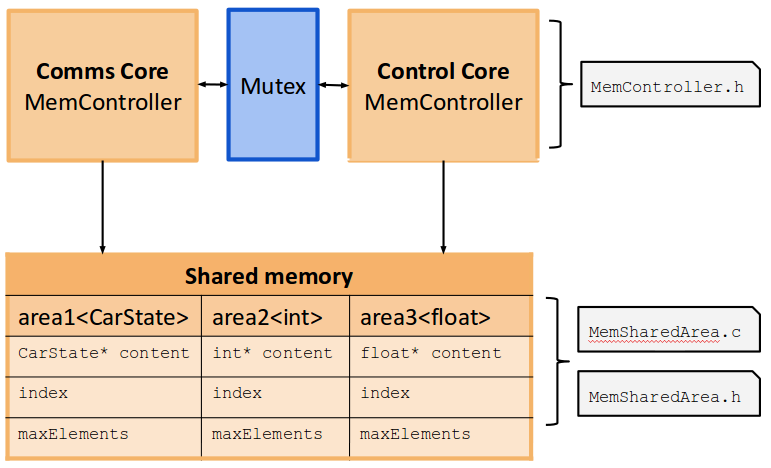
\includegraphics[width=1.0\textwidth]{figures/shared_memory.png}
\end{figure}

\subsection{Location}
The $MemController$ Class resides in $software/shared\_files/MemController.h$. The $MemSharedArea$ is declared in $software/shared\_files/MemSharedArea.h$, with the variable allocation occuring in $MemSharedArea.cpp$.

\subsection{Shared Memory Areas}
The \textbf{$MemSharedArea$} struct (see \ref{sharedmem:code_memsharedarea}) provides a container for managing data in the shared memory. The main goal of the shared memory is to facilitate data exchange between multiple threads/cores.

\begin{lstlisting}[language=C++, label=sharedmem:code_memsharedarea, caption={$MemSharedArea$ structure, the container for shared data. Code found at: $software/ shared\_files/ MemSharedArea.h$}] 
template<typename T>
struct MemSharedArea {
	alt_u32 maxNumElements_u32;
	T * content_a;
	alt_u32 index_u32;
	enum Bufferflags flags_u32;
};
\end{lstlisting}

All containers are declared in $MemSharedArea.c$. Here, the containers are defined and initialised to their default values. In the following snipped, Altera directives are used to instruct the linker to place the variable $AreaCarStateBuffer$ into the hardware memory component titled $.shared\_memory$:
\begin{lstlisting}
CarState AreaCarStateBuffer[BUFFERSIZE_CARSTATE] __attribute__ ((section (".shared_memory")));
\end{lstlisting}
 Note that it is necessary to define both the $MemSharedArea$ container, and the array where the actual content will be stored.

Since the $MemSharedArea$ structure accepts a template argument, any data structure may be stored within the $MemSharedArea$ containers, as long as it can be serialised and there is enough space in memory.


\subsection{Memory controller}
The MemController class provides an interface to access these areas in a safe and ordered fashion. The shared memory area array member is treated as a ring buffer, to allow for a historical retrieval of a certain information stream. 

The primary constructor of a MemController has the following signature:
\begin{lstlisting}
MemController<T>(MemSharedArea<T> * area_p);
\end{lstlisting} 
This creates a MemController object that provides access to the shared memory area $area\_p$. One memory controller is always responsible for just one memory area. Note that the template argument for both the $MemController$ and the $MemSharedArea$ parameter must be the same. 

Currently, there is only one mutex available at the hardware level, so simultaneous access to different shared memory containers is impossible, though it would be safe. A shortened version of the API is shown in snipped \ref{memoryctrl:code_api}.

\begin{lstlisting}[caption={The basic $MemController$ API},label={memoryctrl:code_api}]
// retrieves the newest element from shared memory
T MemController::get();
// retrieves the latest element and keeps the mutex
T MemController::get(bool blocking);   
// deletes all data from the shared memory
void MemController::clear();  
// stores the element T in the memory area
void MemController::push(T element);  
\end{lstlisting}

When using a $MemController$ object, be mindful of the mutex. Most of the mutex management is abstracted away, with it being automatically locked/unlocked as required. However, it is sometimes necessary to retrieve an element from shared memory, make some changes to it and write it back into shared memory, while ensuring that no new elements are written to the buffer in the meantime. 

To do so, use the \lstinline!T MemController::get(bool blocking);! API function. When the parameter is $true$, the mutex will not be released once the element has been retrieved. The core which executed the function will retain mutex ownership until a call to \lstinline!void MemController::push()! is made.

\subsection{Challenges and improvements}
The main challenge of designing the shared memory module primarily lay in the generic design of the data representation in memory and of the $MemController$ class, providing a simple yet powerful framework for others to use. Any serialisable data can be transmitted between threads or physical cores with the current implementation. The API is simple and straightforward to use.

To provide better synchronisation between threads accessing the same shared memory, it would be great if a timestamp/flag could be added to each element in the content buffer. This would ensure that each core knows how many new elements have been added since it last accessed the area and simplify the code when more than one core needs to both read and write to shared memory. One of the challenges with this approach is to synchronise time between the cores. A hardware component may be necessary to achieve this. Currently, the cores are synchronised using indices contained in the data structure written to the shared memory. 

\section{Motor Controller}
The \textbf{Motor Controllers} are aptly named. They control the motor velocities based on a $MotorVelocityMessage$ sent by the central ECU. Last semester's group (WS13/14) did the vast majority of the work on the motor controller code, all credit goes to them. Please see their documentation (found in the repository at $doc/group\_ws13\_14/documentation/documentation.pdf$). 

The following is a short overview of the motor controller, included for completeness' sake.

\subsection{Location}
The software project for the Motor Controllers resides in $software/ Car2X\_nanoMotorCtrl$. The hardware configuration is found here: $hardware/DE0\_Nano.sof$ with the corresponding $.sopcinfo$ file $hardware/DE0\_Nano\_SOPC\_20131216.sopcinfo$

\subsection{Program flow}
The Motor Controller software consists of two logical parts: communication and control. The communications part is responsible for sending message to and receiving messages from the central ECU. These messages include among others, the $WelcomeMessage$ (used during system startup) and the $MotorVelocityMessage$ (contains the desired velocity). The control part is essentially a PID controller that translates the requested motor velocity into PWM signals, and controls the actual velocity using the measurements from an encoder mounted on the motor. The prodedure is shown in snippet \ref{motor:code_mainloop}.

\begin{lstlisting}[label=motor:code_mainloop,caption={The motor controller program in pseudo-code.}]
int main {
  bool startup = false;
  bool newMsg = false;
  double velocity;
  ControlMsg msg;

  while(!startup)  {
    sendWelcomeMsg;
  }
  calibratePIDController;
  
  while(true) {
    if(newMsg) {
      velocity = msg.velocity;
      msg.sendResponse()
    }
    controlMotor(velocity);
  }
}
\end{lstlisting}

\subsection{Changes from previous semester}
Only one major change was made. Previously, the Central ECU would poll the Motor Controllers during system startup with $WelcomeMessages$ until all four Motor Controllers were available. To improve the synchronicity of the system, this behaviour was switched around. The Motor Controllers now periodically send a $WelcomeMessage$ to the Central ECU. Once all Motor Controller have been registered, the Central ECU sends out answers to all client Motor Controllers simultaneously.

\subsection{Challenges and improvements}
We have been unable to use the PID Controller calibration at system startup. The code fails to find correct parameters, resulting in erratic and errorneous behaviour. As a stopgap, the PID values are hardcoded into the software. Debugging was further complicated by the lack of a debugger, thus we were unable to find the true cause for the PID calibration failure.


\section{CarProtocol}
It was part of the work of the previous lab-course group to set up a communication protocol for the car. As the communication was realized using telnet streams, they decided to add another layer over the already existing TCP/IP and telnet protocol layer. This means that the actual protocol for the car is represented by the payload of telnet messages, representing just characters.
\\ \\
In fact, the actual message must be parsed from the incoming telnet  characters. Therefore the so called \glqq CARP\grqq \ or \glqq Car-Protocol\grqq \ consists of packets and messages. Every packet consists of a CARP header and several CARP messages what makes it possible to search the incoming telnet stream for the CARP header and extract all the reqired information about the messages which are part of the specific packet.
\\ \\
For giving a rough idea on how this structure is assembled, here is a figure from Florian Hisch, showing the header-packet-message setup. For a more detailed description have a look at chapter 4.3 of the WS13/14 groups documentation.

\begin{figure}[ht]
	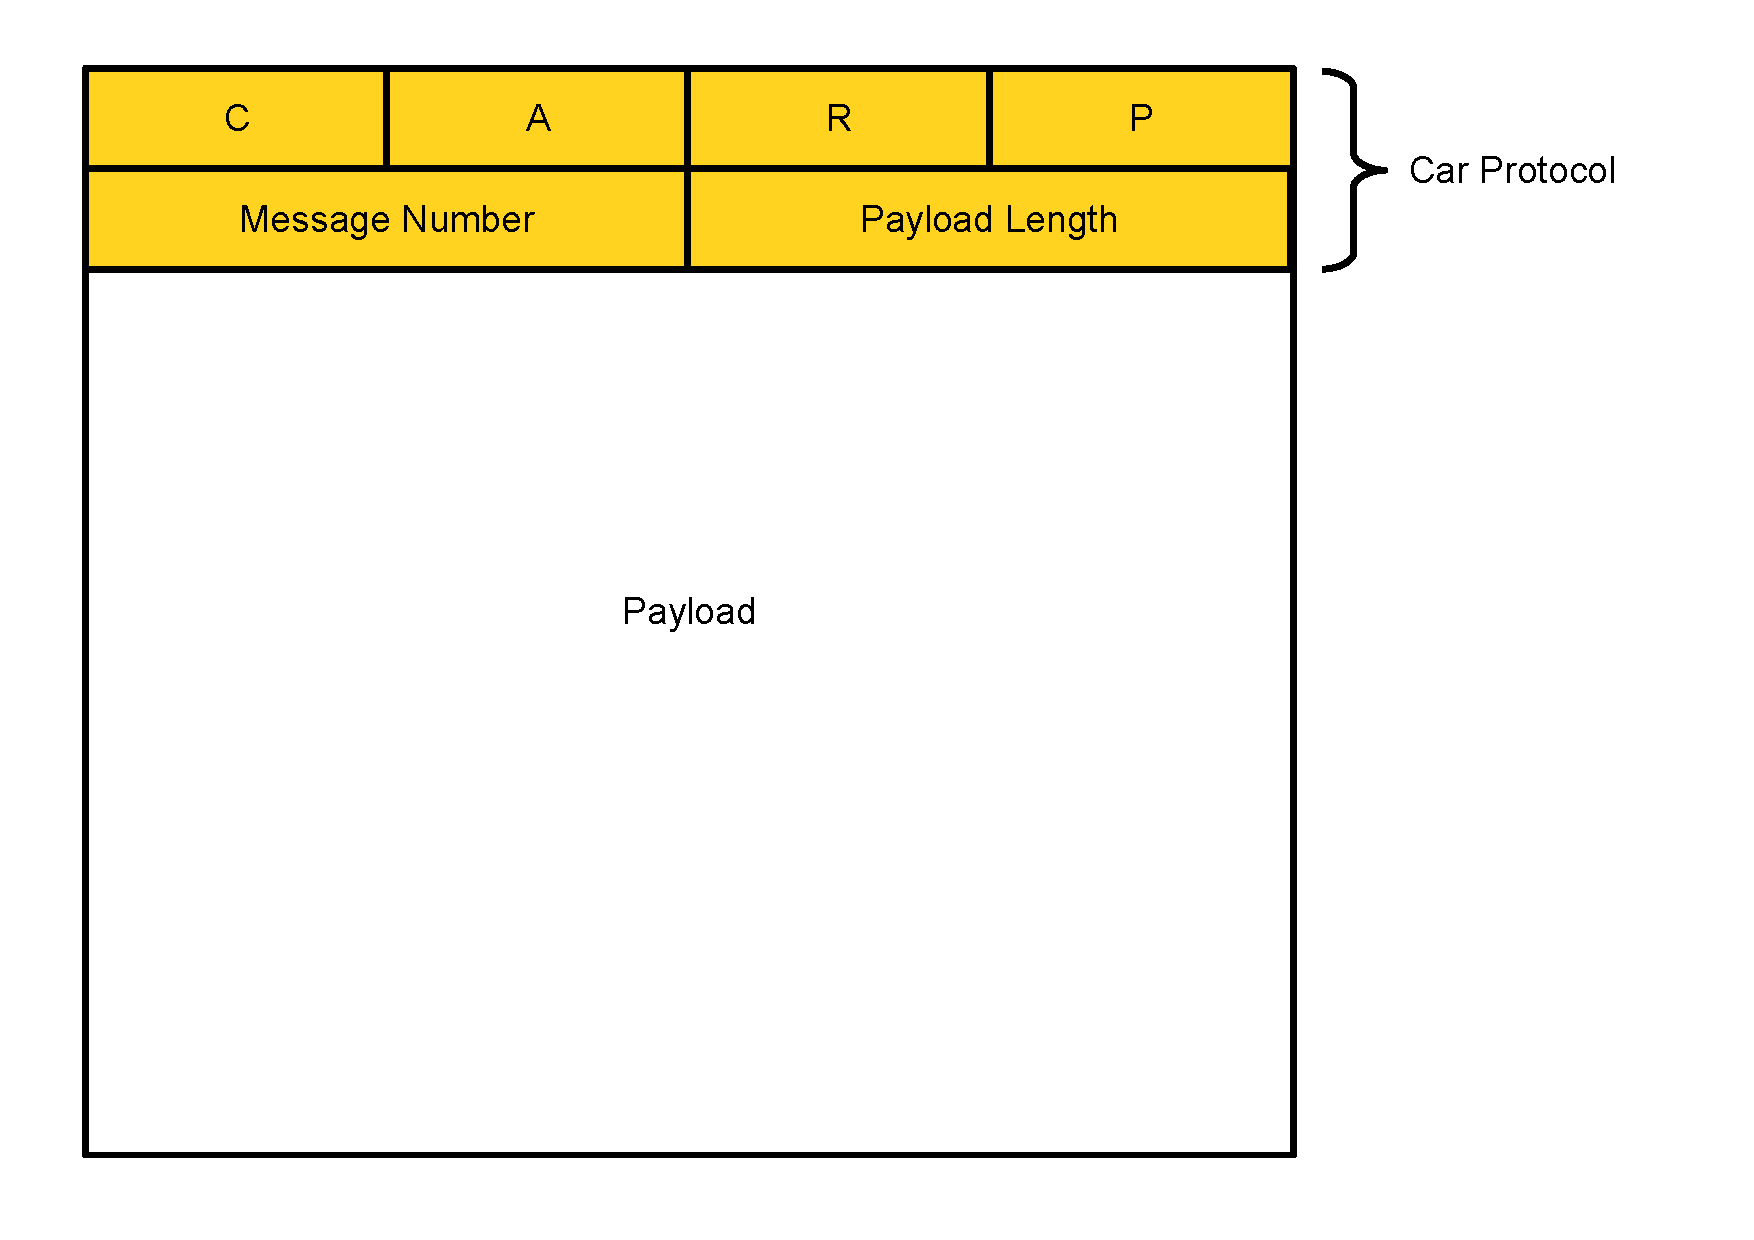
\includegraphics[width=0.5\textwidth]{figures/prot0.pdf}
	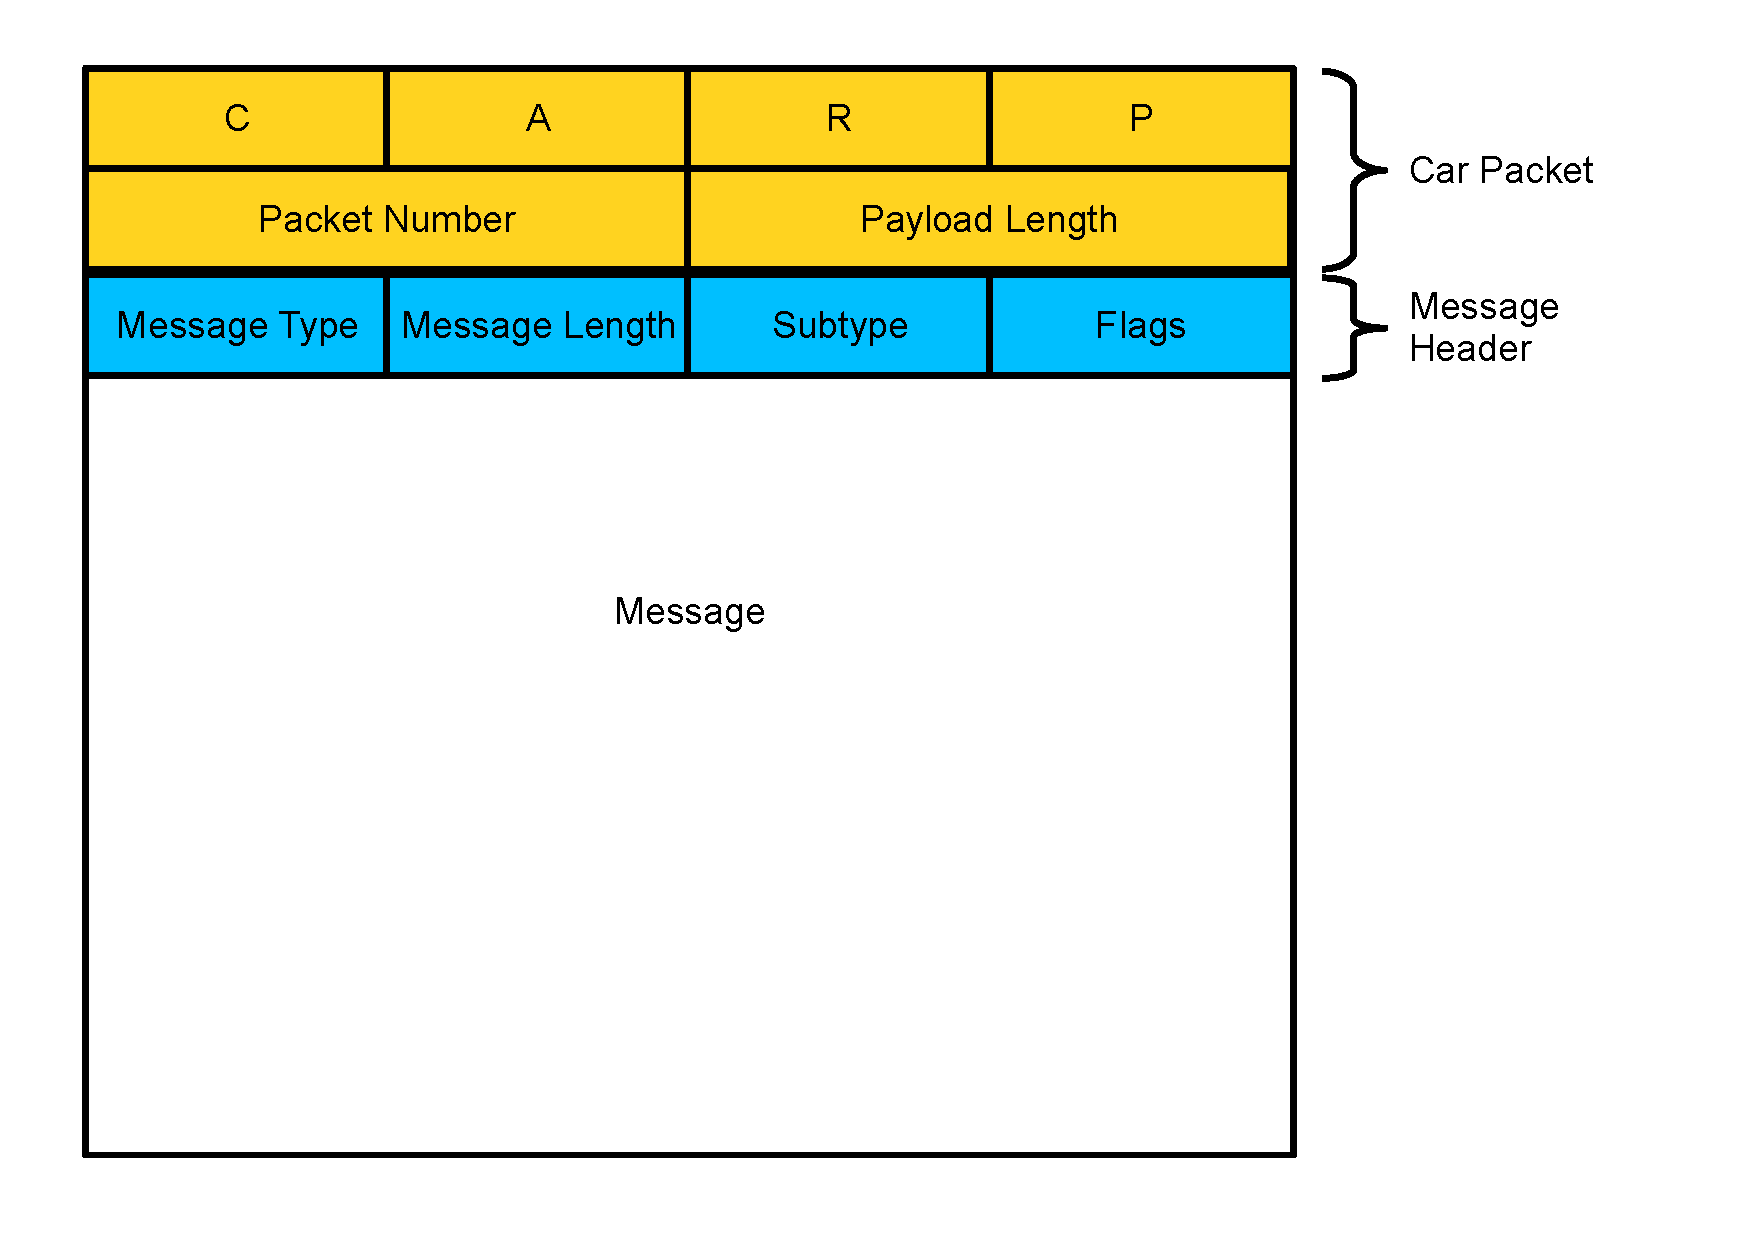
\includegraphics[width=0.5\textwidth]{figures/prot1.pdf}
	\caption{Left: CarProtocol header. Right: CarMessage header.} \label{CarProtocol}
\end{figure}

\section{C2X extensions}
There are basically two types of CAR2X messages. \glqq Polling messages\grqq \ and \glqq Triggering messages\grqq \ which have nearly the same structure as CARP messages. The only difference is that these messages are intended to establish communication with clients other than the core-car-parts. To make it easy to identify CAR2X messages, their 8 bit type-value always has the 4 least significant bits equal to zero: 0xV0  with $0x1\leq V\leq 0xF$.\\ \\
In case of simple \glqq Polling messages\grqq \ that don’t interact with the car state, like the \glqq CInfoStateMessage\grqq \ and the \glqq CInfoSensorMessage\grqq \ which do only read some information out of the current state, there is immediately created and sent an answer message, containing the required data, after the message is executed by the car.\\
The other three messages have an influence on the car state and therefore have to be queued until the car state gets updated. Once the update is there, the main loop of the socketserver checks if the requested state change like for example an emergency brake process has been performed or not, deletes the message from the queue and sends an answer message. Depending on this check the produced answer message contains a different flag: 
\begin{itemize}
\item \glqq A\grqq \ for successful execution(\glqq Answer\grqq)
\item \glqq F\grqq \ for failed execution
\item \glqq O\grqq \ for the message being outdated
\end{itemize}
The main challenge and reason for this check is the fact that communication and state control are performed by different NIOS2 cores. While the state is being updated periodically, incoming messages might arrive more frequent. If for example 3 \glqq CControlMessages\grqq , which contain the information to set the motors to a specific speed, are received within one state update cycle, it is obvious that only the last one should be executed in the new state and the older ones get outdated as soon as a new message of the same type is received. Whenever a message gets queued, and there is already a message in the queue, the outdated one gets immediately answered with an \glqq O\grqq \ flag. This message then is outdated and doesn’t have to be executed any more, since it has been overwritten by the latest message, resulting in only one queued message at maximum for every message type at every state update. For more information about the queueing process read the Communication Core chapter.\\ \\
In the following part all types of CAR2X messages are xplained using examples. Note that there is always the protocol header included.
For answer messages the protocol header consists of CARP, \glqq ControlCoreCounter\grqq ,\glqq CommCoreCounter\grqq \, payloadLength, success-flag and message type.

\subsection*{CEmergencyBrakeMessage}
Example packet sent to the car:\\
\resizebox{\linewidth}{!}{
\renewcommand{\arraystretch}{1.5}
\begin{tabular}{|c||c|c|c|c|c|c|c|c|c|c|}
\hline 
\rule[-1ex]{0pt}{2.5ex} Byte & 1 & 2 & 3 & 4 & 5 + 6 & 7 + 8 & 9 & 10 & 11 & 12 \\ 
\hline 
\rule[-1ex]{0pt}{2.5ex} Inhalt & C & A & R & P & PacketID & PayloadLength: 0x04 & Type: 0x20 & Length: 0x04 & Subtype: 0x0 & Flags: 0x0 \\ 
\hline 
\end{tabular}} \\
\newline
\newline
After receiving this message, the control core is requested to change the car state into emergency braking and this message is queued to wait for the next state update, or being outdated.\\
\newline
The payload of the answer consists of the PacketNumber of the received message.\\
\newline
Example answer message sent by the car:\\
\resizebox{\linewidth}{!}{
\renewcommand{\arraystretch}{1.5}
\begin{tabular}{|c||c|c|c|c|c|c|c|c|c|c|}
\hline 
\rule[-1ex]{0pt}{2.5ex} Byte & 1 & 2 & 3 & 4 & 5 - 8 & 9 - 12 & 13 - 16 & 17 & 18 & 19 + 20 \\ 
\hline 
\rule[-1ex]{0pt}{2.5ex} Inhalt & C & A & R & P & ControlCoreCounter & CommCoreCounter & PayloadLength & Success flag (‘A’,’F’,’O’) & Type: 0x20 & PacketID of the received message \\ 
\hline 
\end{tabular}}

\subsection*{CControlMessage}
Example packet sent to the car:\\
\resizebox{\linewidth}{!}{
\renewcommand{\arraystretch}{1.5}
\begin{tabular}{|c||c|c|c|c|c|c|c|c|c|c|c|c|c|c|}
\hline 
\rule[-1ex]{0pt}{2.5ex} Byte & 1 & 2 & 3 & 4 & 5 + 6 & 7 + 8 & 9 & 10 & 11 & 12 & 13 + 14 & 15 + 16 & 17 + 18 & 19 + 20 \\ 
\hline 
\rule[-1ex]{0pt}{2.5ex} Inhalt & C & A & R & P & PacketID & PayloadLength: 0x0C & Type: 0x30 & Length: 0x0C & Subtype: 0x0 & Flags: 0x0 & V1 & V2 & V3 & V4 \\ 
\hline 
\end{tabular}} \\
\newline
\newline
After receiving this message, the control core is requested to set the specified motor velocities (V1...4 as 16-bit values), specified in the payload. It has to be mentioned that in case the sender of this message is not registered as the current source of control, the message is not queued but immediately replied as failed because the sender is not allowed to control the car.
But if the control is allowed, this message is queued to wait for the next state update, or getting out of date.\\
\newline
Example answer message sent by the car:\\
\resizebox{\linewidth}{!}{
\renewcommand{\arraystretch}{1.5}
\begin{tabular}{|c||c|c|c|c|c|c|c|c|c|c|c|c|c|c|}
\hline 
\rule[-1ex]{0pt}{2.5ex} Byte & 1 & 2 & 3 & 4 & 5 - 8 & 9 - 12 & 13 - 16 & 17 & 18 & 19 + 20 & 21 + 22 & 23 + 24 & 25 + 26 & 17 + 28\\ 
\hline 
\rule[-1ex]{0pt}{2.5ex} Inhalt & C & A & R & P & ControlCoreCounter & CommCoreCounter & PayloadLength & Success flag (‘A’,’F’,’O’) & Type: 0x30 & PacketID of the received message & V1 & V2 & V3 & V4\\ 
\hline 
\end{tabular}}\\
\newline
V1 to V4 are now standing for the current desired motor speed values delivered to the specific PWM motor controllers. In case of a successful message, they are equal to the requested values of the message, sent to the car, otherwise they differ and the message is answered as \glqq failed\grqq , giving the controlling unit feedback about the current state of the car, to let it know what might have failed.

\subsection*{CRemoteControlMessage}
Example packet sent to the car:\\
\resizebox{\linewidth}{!}{
\renewcommand{\arraystretch}{1.5}
\begin{tabular}{|c||c|c|c|c|c|c|c|c|c|c|c|c|c|c|}
\hline 
\rule[-1ex]{0pt}{2.5ex} Byte & 1 & 2 & 3 & 4 & 5 + 6 & 7 + 8 & 9 & 10 & 11 & 12 & 13 & 14 & 15 & 16 \\ 
\hline 
\rule[-1ex]{0pt}{2.5ex} Inhalt & C & A & R & P & PacketID & PayloadLength: 0x08 & Type: 0x60 & Length: 0x08 & Subtype: 0x0 & Flags: 0x0 & IP1 & IP2 & IP3 & IP4 \\ 
\hline 
\end{tabular}} \\
\newline
\newline
The payload of this message contains the IP of a source which should be allowed to control the car by using \glqq CControlMessages\grqq . Per default this source is the unit inside of the car featuring the ImageProcessingUnit with its IP 192.168.0.110. In the standard state of the car \glqq AutoDrive\grqq , the car is controlled from this IP by \glqq CControlMessages\grqq . By sending a \glqq CRemoteControlMessage\grqq \ to the car containing a different IP, the car is requested to set its state to \glqq ManualDrive\grqq \ with the new source IP locked for \glqq CControlMessages\grqq . Sending 0.0.0.0 as new IP will set the car back to \glqq AutoDrive\grqq , using the ImageProcessing IP again.
As before, the answer gets queued until the state is updated for the next time.\\
\newline
Example answer message sent by the car:\\
\resizebox{\linewidth}{!}{
\renewcommand{\arraystretch}{1.5}
\begin{tabular}{|c||c|c|c|c|c|c|c|c|c|c|c|c|c|c|}
\hline 
\rule[-1ex]{0pt}{2.5ex} Byte & 1 & 2 & 3 & 4 & 5 - 8 & 9 - 12 & 13 - 16 & 17 & 18 & 19 + 20 & 21 + 22 & 23 + 24 & 25 + 26 & 17 + 28\\ 
\hline 
\rule[-1ex]{0pt}{2.5ex} Inhalt & C & A & R & P & ControlCoreCounter & CommCoreCounter & PayloadLength & Success flag (‘A’,’F’,’O’) & Type: 0x60 & PacketID of the received message & IP1 & IP2 & IP3 & IP4\\ 
\hline 
\end{tabular}}\\
\newline
IP1 to IP4 are the current state values of the locked IP. In case of success they equal the requested one, otherwise they give the feedback about who is currently controlling the car.

\subsection*{CInfoStateMessage}
Example packet sent to the car:\\
\resizebox{\linewidth}{!}{
\renewcommand{\arraystretch}{1.5}
\begin{tabular}{|c||c|c|c|c|c|c|c|c|c|c|c|c|c|c|}
\hline 
\rule[-1ex]{0pt}{2.5ex} Byte & 1 & 2 & 3 & 4 & 5 + 6 & 7 + 8 & 9 & 10 & 11 & 12 & 13 & 14 & 15 & 16 \\ 
\hline 
\rule[-1ex]{0pt}{2.5ex} Inhalt & C & A & R & P & PacketID & PayloadLength: 0x04 & Type: 0x40 & Length: 0x04 & Subtype: 0x0 & Flags: 0x0\\ 
\hline 
\end{tabular}} \\
\newline
\newline
This message just polls the current state information from the car. It is answered immediately and thus has not to be queued. The answer always contains the \glqq A\grqq \ flag for success and features the biggest part of the state object from the shared memory as its payload. It can be used for debugging purposes or by the ImageProcessing unit or a station as additional odometry feedback\\
\newline
Example answer message sent by the car:\\
\resizebox{\linewidth}{!}{
\renewcommand{\arraystretch}{1.5}
\begin{tabular}{|c||c|c|c|c|c|c|c|c|c|c|c|c|c|c|c|c|c|c|c|c|c|c|c|c|c|c|}
\hline 
\rule[-1ex]{0pt}{2.5ex} Byte & 1 & 2 & 3 & 4 & 5 - 8 & 9 - 12 & 13 - 16 & 17 & 18 & 19 + 20 & 21 - 24 & 25 & 26 & 27 & 28 & 29 & 30 & 31 & 32 & 33 & 34 & 35 - 56 & 57 - 78 & 79 - 100 & 101 - 122 & 123 - 130 \\ 
\hline 
\rule[-1ex]{0pt}{2.5ex} Inhalt & C & A & R & P & ControlCoreCounter & CommCoreCounter & PayloadLength & Success flag (‘A’,’F’,’O’) & Type: 0x40 & PacketID of the received message & iMaxSpeed & IP1 & IP2 & IP3 & IP4 & reqIP1 & reqIP2 & reqIP3 & reqIP4 & currMode & reqMode & 1st ECU state & 2nd ECU state & 3rd ECU state & 4th ECU state & reqVelocity\\ 
\hline 
\end{tabular}}\\
\newline
As \glqq ControlCoreCounter\grqq \ and \glqq CommCoreCounter\grqq \ are already part of the answer header while also beeing part of the car-state, they are excluded from the payload. Its the same for the sensor values which are polled by the \glqq CInfoSensorMessage\grqq seperately to safe bandwidth.

\subsection*{CInfoSensorMessage}
Example packet sent to the car:\\
\resizebox{\linewidth}{!}{
\renewcommand{\arraystretch}{1.5}
\begin{tabular}{|c||c|c|c|c|c|c|c|c|c|c|c|c|c|c|}
\hline 
\rule[-1ex]{0pt}{2.5ex} Byte & 1 & 2 & 3 & 4 & 5 + 6 & 7 + 8 & 9 & 10 & 11 & 12 & 13 & 14 & 15 & 16 \\ 
\hline 
\rule[-1ex]{0pt}{2.5ex} Inhalt & C & A & R & P & PacketID & PayloadLength: 0x04 & Type: 0x50 & Length: 0x04 & Subtype: 0x0 & Flags: 0x0S\\ 
\hline 
\end{tabular}} \\
\newline
\newline
This message just polls the current sensor information from the car state. It is answered immediately and thus has not to be queued. The answer always contains the \glqq A\grqq flag for success and features the whole sensor information which are part of the car state. This message can be used to access the sensor data. Note that currently there is no sensor hardware connected and there is still no implementation to get the sensor information from this missing hardware. On the other hand, the state object already contains memory to store this data which is read out by one of these messages. The polling interface by CAR2X messages is completely working for an assumed amount of 2 sensors but will always deliver no information until the internal sensor read out will be implemented.\\
\newline
Example answer message sent by the car:\\
\resizebox{\linewidth}{!}{
\renewcommand{\arraystretch}{1.5}
\begin{tabular}{|c||c|c|c|c|c|c|c|c|c|c|c|c|c|c|}
\hline 
\rule[-1ex]{0pt}{2.5ex} Byte & 1 & 2 & 3 & 4 & 5 - 8 & 9 - 12 & 13 - 16 & 17 & 18 & 19 + 20 & 21 - 24 & 25 - 28\\ 
\hline 
\rule[-1ex]{0pt}{2.5ex} Inhalt & C & A & R & P & ControlCoreCounter & CommCoreCounter & PayloadLength & Success flag (‘A’,’F’,’O’) & Type: 0x50 & PacketID of the received message & Sensor 1 Value & Sensor 2 Value\\ 
\hline 
\end{tabular}}\\
\newline
